%!TEX program = xelatex
\documentclass[12pt, a4paper]{article}
\usepackage[utf8]{inputenc}
\usepackage[russian]{babel}
\usepackage{pscyr}

\usepackage{xifthen}
\usepackage{parskip}
\usepackage{hyperref}
\usepackage[top=0.7in, bottom=1in, left=0.6in, right=0.6in]{geometry}
\usepackage{setspace}

\usepackage{amsmath}
\usepackage{MnSymbol}
\usepackage{amsthm}
\usepackage{mathtools}

\usepackage{algorithm}
\usepackage[noend]{algpseudocode}



\linespread{1.2}
\setlength{\parskip}{0pt}

\renewcommand\familydefault{\sfdefault}


% Stuff related to homework specific documents
\newcounter{MyTaskCounter}
\newcounter{MyTaskSectionCounter}
\newcommand{\tasksection}[1]{
	\stepcounter{MyTaskSectionCounter}
	\setcounter{MyTaskCounter}{0}
	\ifthenelse{\equal{#1}{}}{}{
	{\hfill\\[0.2in] \Large \textbf{\theMyTaskSectionCounter \enspace #1} \hfill\\[0.1in]}}
}

\newcommand{\task}[1]{
	\stepcounter{MyTaskCounter}
	\hfill\\[0.1in]
	\ifthenelse{\equal{\theMyTaskSectionCounter}{0}}{
	   \textbf{\large Задача №\theMyTaskCounter}
	}{
	   \textbf{\large Задача №\theMyTaskSectionCounter.\theMyTaskCounter}
	}
	\ifthenelse{\equal{#1}{}}{}{{\normalsize (#1)}}
	\hfill\\[0.05in]
}

% Math and algorithms

\makeatletter
\renewcommand{\ALG@name}{Алгоритм}
\renewcommand{\listalgorithmname}{Список алгроитмов}

\newenvironment{procedure}[1]
  {\renewcommand*{\ALG@name}{Процедура}
  \algorithm\renewcommand{\thealgorithm}{\thechapter.\arabic{algorithm} #1}}
  {\endalgorithm}

\makeatother

\algrenewcommand\algorithmicrequire{\textbf{Вход:}}
\algrenewcommand\algorithmicensure{\textbf{Выход:}}
\algnewcommand\True{\textbf{true}\space}
\algnewcommand\False{\textbf{false}\space}
\algnewcommand\And{\textbf{and}\space}

\newcommand{\xfor}[3]{#1 \textbf{from} #2 \textbf{to} #3}
\newcommand{\xassign}[2]{\State #1 $\leftarrow$ #2}
\newcommand{\xstate}[1]{\State #1}
\newcommand{\xreturn}[1]{\xstate{\textbf{return} #1}}

\DeclarePairedDelimiter\ceil{\lceil}{\rceil}
\DeclarePairedDelimiter\floor{\lfloor}{\rfloor}

\newcommand{\bigO}[1]{\mathcal{O}\left(#1\right)}

\makeatletter
\def\input@path{{./pics/}}
\makeatother
\graphicspath{{./pics/}}

\title{Домашнее задание №3 \\ Информационный поиск. 6 курс. Осенний семестр.}
\author{Горбунов Егор Алексеевич}
\date{11 ноября 2016 г.}
\begin{document}
\maketitle

\begin{task}[1]
Перед вами матрица смежности <<термин-документ>>, описывающая некую коллекцию (строки -- термы, столбцы -- документы):
\begin{equation*}
	C = 
	\begin{pmatrix}
	1 & 1 \\
	0 & 1 \\
	1 & 0
	\end{pmatrix}
\end{equation*}
\begin{enumerate}
	\item Вычислите матрицу совместной встречаемости $CC^T$. Что собой представляют диагональные элементы этой матрицы?
	\item Убедитесь, что сингулярное разложение матрицы $C$ выглядит следующим образом:
	\begin{equation*}
		U = 
		\begin{pmatrix}
		 -0.816 & 0.000 \\
		 -0.408 & -0.707 \\
		 -0.408 & 0.707
		\end{pmatrix}
		,
		\Sigma =
		\begin{pmatrix}
		1.732 & 0.000 \\
		0.000 & 1.000
		\end{pmatrix}
		,
		V^T = 
		\begin{pmatrix}
		-0.707 & -0.707 \\
		0.707 & -0.707
		\end{pmatrix}
	\end{equation*}
	\item Что собой представляют элементы матрицы $C^TC$? \label{t1:item3} 
\end{enumerate}
\end{task}
\begin{solution}
\begin{enumerate}
	\item Обозначим вектора слов:
	\begin{equation*}
		w_1 = \mmat{1\\1},
		w_2 = \mmat{0\\1},
		w_3 = \mmat{1\\0}
	\end{equation*}
	Элемент вектора $w_i[j]$ обозначает, встретилось ли слово $w_i$ в документе $D_j$.\\
	Тогда матрица совместной встречаемости ($\cdot$ -- скалярное произведене, dot product):
	\begin{equation*}
		CC^T = 
		\begin{pmatrix}
		w_1^T \\
		w_2^T \\
		w_3^T
		\end{pmatrix}
		\begin{pmatrix}
		w_1 & w_2 & w_3
		\end{pmatrix}^T
		=
		\begin{pmatrix}
		w_1 \\ w_2 \\ w_3
		\end{pmatrix}
		\begin{pmatrix}
		w_1 & w_2 & w_3
		\end{pmatrix}
		=
		\begin{pmatrix}
		w_1 \cdot w_1 && w_1 \cdot w_2 && w_1 \cdot w_3 \\
		w_2 \cdot w_1 && w_2 \cdot w_2 && w_2 \cdot w_3 \\
		w_3 \cdot w_1 && w_3 \cdot w_2 && w_3 \cdot w_3
		\end{pmatrix}
	\end{equation*}
	Откуда:
	\begin{equation*}
	CC^T=
	\begin{pmatrix}
	2 & 1 & 1 \\
	1 & 1 & 0 \\
	1 & 0 & 1 
	\end{pmatrix}
	\end{equation*}
	В силу того, что $w_i$ --- вектор над $\xbrace{1, 0}$, видно, что диагональный элемент матрицы $CC^T[i, i]$ равен числу документов коллекции, в которых встретилось слово $w_i$. Вообще: $CC^T[i, j]$ -- это скалярное произведение $w_i \cdot w_j$, которое
	представляет из себя сумму элементов вектора, в котором $1$ стоят на таких позициях $k$, что $w_i[k] = w_j[k] = 1$. Таким образом сумма элементов данного вектора будет равна число документов, в которых одновременно встречается как слово $w_i$ так и слово $w_j$.
	\item Перемножив данные матрицы получим:
	\begin{equation*}
	U\Sigma V^T = 
	\begin{pmatrix}
		0.9992 & 0.9992 \\
		-0.0002 & 0.9994 \\ 
        0.9994 & -0.0002
	\end{pmatrix}
	\end{equation*}
	Вообщем-то похоже, но с погрешностью. Как минимум по-этому SVD стоит пересчитать руками =) Также, по определению сингулярного разложения исходная матрица раскладывается в произведение унитарной, диагональной (из ненулевых сингулярных чисел) и ещё одной унитарной матрицы. Матрица $U$, приведённая в задании не является унитарной, как минимум потому, что не является квадратной. Таким образом приведённое разложение нельзя называть сингулярным в каноническом понимании (как я понимаю), хотя это и не означает, что такое разложение неверно и его нельзя использовать для решения содержательных задач поиска. Поэтому найдём сингулярное разложение матрицы $C$ своими силами.
	Будем искать матрицы $U$, $V$ и $\Sigma$, что $U$ имеет размер $3\times3$, $\Sigma$ $3\times2$, а $V$ $2 \times 2$. В силу унитарности матриц $U$ и $V$ можем записать следующее:
	\begin{align*}
		& U^T U = UU^T = V^TV = VV^T = I \\
		& CC^T = U\Sigma V^T V\Sigma^TU^T = U\Sigma\Sigma^TU^T \\
		& C^TC = V\Sigma^TU^TU\Sigma V^T = V\Sigma^T\Sigma V^T 
	\end{align*}
	Тут матрица $\Sigma^T \Sigma = \Sigma\Sigma^T = \Lambda$ --- это квадратная диагональная матрица $3\times3$ (на диагонали могут быть нули).\\
	Откуда мы получаем, домножая справа обе части на нужные $U$ в одном уравнении и на $V$ в другом:
	\begin{align*}
		& (CC^T)U = U\Lambda \\
		& (C^TC)V = V\Lambda
	\end{align*}
	Можно переписать это так:
	\begin{align*}
		(CC^T)\vec{u_i} &= \vec{u_i}\lambda_i,\ \text{для всех столбцов $u_i$ матрицы $U$} \\
		(C^TC)\vec{v_i} &= \vec{v_i}\lambda_i,\ \text{для всех столбцов $v_i$ матрицы $V$} \\
		\Lambda &= 
		\begin{pmatrix}
			\lambda_1 & 0 & 0 \\
			0 & \lambda_2 & 0 \\
			0 & 0 & \lambda_3
		\end{pmatrix},
		\ \Sigma[i][i] = \sqrt{\lambda_i}
	\end{align*}
	Видим, что собственные числа (ненулевые!) матриц $C^TC$ и $CC^T$ совпадают и равны квадратам искомых сингулярных чисел, составляющих $\Sigma$, а столбцы матрицы $V$ --- собственные вектора $C^TC$ и столбцы $U$ --- собственные вектора $CC^T$.
	Таким образом нам нужно отыскать собственные числа и вектора матриц:
	\begin{equation*}
	CC^T=
	\begin{pmatrix}
	2 & 1 & 1 \\
	1 & 1 & 0 \\
	1 & 0 & 1 
	\end{pmatrix},\
	C^TC=
	\begin{pmatrix}
	1 & 0 & 1 \\
	1 & 1 & 0 
	\end{pmatrix}
	\begin{pmatrix}
	1 & 1 \\
	0 & 1 \\
	1 & 0
	\end{pmatrix}
	=
	\begin{pmatrix}
	2 & 1 \\
	1 & 2 
	\end{pmatrix}
	\end{equation*}
	Начнём с собственных чисел. Ищем их через характеристические многочлены (приравнивая их к $0$, почему так делается я не поясняю, т.к. это за рамками курса):
	\begin{align*}
	&det
	\begin{pmatrix}
	2 - \lambda & 1 & 1 \\
	1 & 1 - \lambda & 0 \\
	1 & 0 & 1 - \lambda
	\end{pmatrix}
	= (2-\lambda)(1-\lambda)^2-(1-\lambda)-(1-\lambda)=\lambda(1-\lambda)(\lambda-3)
	 \\
	&\Lambda = 
	\begin{pmatrix}
	3 & 0 & 0 \\
	0 & 1 & 0 \\
	0 & 0 & 0
	\end{pmatrix}
	\end{align*}
	Чтобы получить $U$ и $V$ теперь нужно найти собственные векторы соответствующие собственным числам $3$ и $1$ матриц 
	$CC^T$ и $C^TC$. Теперь уже совсем очевидно, что столбец $\vec{u_3}$ может быть произвольным собственным вектором (соответствует с.ч. $0$) и роли он в разложении играть не будет. Для векторов получаем следующие системы (матрица системы та же, что под $det$ выше, но с уже подставленными $\lambda$) ($u_1, v_1$ соответствует $\lambda = 3$, $u_2, v_2$ соотв. $\lambda = 1$). Т.к. итоговые матрицы $U$ и $V$ должны быть унитарными, то вектора необходимо нормализовать.
	\begin{align*}
	\begin{cases}
	-u_{11} + u_{12} + u_{13} = 0 \\
	u_{11} - 2u_{12} = 0 \\
	u_{11} - 2u_{13} = 0
	\end{cases}
	\text{, откуда легко подобрать } \mmat{-2 \\ -1 \\ -1} \Rightarrow u_1 = \frac{1}{\sqrt{6}}\mmat{-2 \\ -1 \\ -1}\\
	\begin{cases}
	u_{21} + u_{22} + u_{23} = 0 \\
	u_{21} = 0 \\
	u_{21} = 0
	\end{cases}
	\text{, откуда легко подобрать } \mmat{0 \\ -1 \\ 1} \Rightarrow u_2 = \frac{1}{\sqrt{2}}\mmat{0 \\ -1 \\ 1}
	\end{align*}
	Аналогично можно подобрать собственный вектор для $\lambda_3 = 0$: $u_3 = \frac{1}{\sqrt{3}}\mmat{-1 \\ 1 \\ 1}$.
	Для $v_i$:
		\begin{align*}
	\begin{cases}
	-v_{11} + v_{12} = 0 \\
	v_{11} - v_{12} = 0 
	\end{cases}
	\text{, откуда легко подобрать } \mmat{-1 \\ -1} \Rightarrow v_1 = \frac{1}{\sqrt{2}}\mmat{-1 \\ -1}\\
	\begin{cases}
	v_{21} + v_{22} = 0 \\
	v_{21} + v_{22}= 0 
	\end{cases}
	\text{, откуда легко подобрать } \mmat{1 \\ -1} \Rightarrow v_2 = \frac{1}{\sqrt{2}}\mmat{1 \\ -1}
	\end{align*}
	Итого мы получили искомое разложение:
	\begin{align*}
	U &= 
	\begin{pmatrix}
	u_1 && u_2 && u_3 
	\end{pmatrix}
	=
	\begin{pmatrix}
	\frac{-2}{\sqrt{6}} & 0 & \frac{-1}{\sqrt{3}} \\
	\frac{-1}{\sqrt{6}} & \frac{-1}{\sqrt{2}} & \frac{1}{\sqrt{3}} \\
	\frac{-1}{\sqrt{6}} & \frac{1}{\sqrt{2}} & \frac{1}{\sqrt{3}}
	\end{pmatrix} \\
	V^T &=
	\begin{pmatrix}
	v_1^T \\
	v_2^T 
	\end{pmatrix}
	=
	\begin{pmatrix}
	\frac{-1}{\sqrt{2}} & \frac{-1}{\sqrt{2}} \\
	\frac{1}{\sqrt{2}} & \frac{-1}{\sqrt{2}}
	\end{pmatrix} \\
	\Sigma &= 
	\begin{pmatrix}
		\sqrt{3} & 0 \\
		0 & 1 \\
		0 & 0
	\end{pmatrix}
	\end{align*}
	Конечно, при вычислении собственных векторов я выбирал те знаки, которые бы соответствовали тому, что дано в задании =)
	Теперь, если перевести все значения в десятичные дроби легко увидеть, что полученные матрицы совпадают (если округлить до нужного числа знаков), кроме того, что вычисленная явно $U$ является честно унитарной, хоть на дальнейшие выкладки (например, при вычислении новых векторов для документов (LSA)) это не влияет. Таким образом ответ: всё ок, убедились в том, что это сингулярное разложение (но не уд. определению).

	\item Аналогично пункту (a) введём вектора документов:
	\begin{align*}
	D_1 = \mmat{1 \\ 0 \\ 1}
	D_2 = \mmat{1 \\ 1 \\ 0}
	\end{align*}
	Тут если $D_i[k] = 1$, то терм $w_k$ встретился в документе $D_i$.\\
	Тогда получим:
	\begin{equation*}
	C^TC =
	\begin{pmatrix}
	D_1 \cdot D_1 & D_1 \cdot D_2 \\
	D_2 \cdot D_1 & D_2 \cdot D_2
	\end{pmatrix}
	=
	\begin{pmatrix}
	2 & 1 \\
	1 & 2 
	\end{pmatrix}
	\end{equation*}
	Откуда легко видеть, опять же аналогично первому пункту задания, что $C^TC[i, j]$ --- это число термов, которые \emph{одновременно} встречаются в документах $D_i$ и $D_j$, т.е. это мощность пересечения мешков слов для документов $D_i$ и $D_j$. Ещё можно написать, что $C^TC[i, j] = sim(D_i, D_j) ||D_i|| ||D_j||$.
\end{enumerate}
\end{solution}

\begin{task}[2]
Для чего используются распределения Дирихле $Dir(\vec{\alpha})$ и $Dir(\vec{\beta})$ в тематических
моделях? Что контролируют параметры $\vec{\alpha}$ и $\vec{\beta}$? Какие значения этих параметром имеет смысл использовать и почему?
\end{task}
\begin{solution}
Начнём с того, что опишем, что из себя представляет распределение Дирихле. 
Распределение Дирихле -- это \emph{сопряжённое априорное распределение} для мультиномиального распределения. Функция плотности вероятности распределения Дирихле:
\begin{align*}
Dir(\vec{p} | \vec{\alpha}) &= \frac{1}{B(\vec{\alpha})}\prod_{i = 1}^{m}{p_i^{\alpha_i - 1}}, \text{ где } \vec{p} = \xbrace{p_1, \ldots, p_m}, \vec{\alpha} = \xbrace{\alpha_1, \ldots, \alpha_m} \\
B(\vec{\alpha}) &= \frac{\prod_{i = 1}^m{\Gamma(\alpha_i)}}{\Gamma(\sum_{i=1}^m{\alpha_i})} = \xbracket{\text{при натуральных } \alpha_i} = \frac{\prod_{i=1}^m{(\alpha_i-1)!}}{(\sum_{i=1}^m{\alpha_i}-1)!}
\end{align*}
$B(\vec{\alpha})$ --- бета-функция, при раскрытии которой выше было использовано, что $\Gamma(x)$ (гамма-функция) --- это обобщение факториала. Носителем распределения Дирихле, т.е. функции $Dir$ является множество векторов $\vec{p}$ таких, что $p_i \in (0, 1)$ и $\sum{p_i} = 1$, т.е. сгенерировав случайный вектор $\vec{p}$ из распределения Дирихле, мы можем интерпретировать его как набор вероятностей --- параметров мультиномиального распределения. Таким образом распределение Дирихле является \emph{распределением над распределениями}.
Можно посчитать математическое ожидание и дисперсию $p_i$ ($\vec{p} \sim Dir(\alpha)$) (считать не будем, а посмотрим в википедии):
\begin{align}
	\label{dir_exp} E\xbracket{p_i} &= \frac{\alpha_i}{\sum_k{\alpha_k}}\\
	\label{dir_var} Var\xbracket{p_i} &= \frac{\alpha_i(\sum_k{\alpha_k} - \alpha_i)}{\xparen{\sum_k{\alpha_k}}^2(\sum_k{\alpha_k} + 1)}
\end{align}

\begin{itemize}
	\item Для чего используются $Dir(\vec{\alpha})$ и $Dir(\vec{\beta})$? Тематические модели пытаются вероятностно описать факт того, что документ может одновременно содержать несколько тем (например, статья может рассказывать о животных с точки зрения биологии, географии и истории). При построении тематических модели документа (модель у нас генеративная, как на лекции) нужно понять:
	\begin{enumerate}
		\item Каково распределение тем в документе? Т.е. выбрать набор вероятностей $\vec{p} = \xbrace{p_1, p_2, \ldots, p_k}$, где $p_j$ --- вероятность $j$-ой темы. Тем всего $k$.
		\item Каково распределение слов в конкретной теме $i$? Т.е. набор вероятностей $\vec{q} = \xbrace{q_1, q_2, \ldots, q_m}$, где $m$ --- размер словаря.
	\end{enumerate}
	Далее, имя $\vec{p}$ можно сгенерировать тему --- число от $1$ до $k$, а после из темы выбрать слово по распределению вероятностей $\vec{q}$.\\
	Так вот именно для ответа на вопросы <<каково распределение тем в документе?>> и <<каково распределение слов в конкретной теме?>> и используются в тематических моделях распределения, соответственно, $Dir(\vec{\alpha})$ и $Dir(\vec{\beta})$. Т.е. в генеративной модели документа первоочерёдно происходит сэмплирование из этих распределений для дальнейшей генерации документа.

	\item Что контролируют параметры $\alpha$ и $\beta$? Тут, как мне кажется, достаточно ответить на вопрос в общем: что контролируют параметры распределения Дирихле? Пускай у нас $k$ параметров, т.е. $\alpha = \xbrace{\alpha_1, \ldots, \alpha_k}$, т.е. $Dir(\vec{\alpha})$ генерирует $k$ вероятностей. Коротко: параметры $\vec{\alpha}$ контролируют свойства генерируемого вероятностного распределения $\vec{p}$, т.е. то, как вероятность распределяется по <<исходам>> (или классам) $\xbrace{1, \ldots, k}$.

	Длинно: посмотрим на выражения математического ожидания~\ref{dir_exp} и дисперсии~\ref{dir_var} для распределения Дирихле. Видим, что:
	\begin{itemize}
		\item чем больше какой-то параметр $\alpha_i$, тем больше ожидаемая вероятность <<исхода>> (класса) $i$. Поэтому $\alpha_i$ можно называть весом класса $i$. На рисунке~\ref{fig:dir_inc_w} показан сгенерированный (используя python+numpy+matplotlib) набор вероятностей для $50$ классов, в подтверждение этих рассуждений.
	\begin{figure}[ht!]
	\centering
	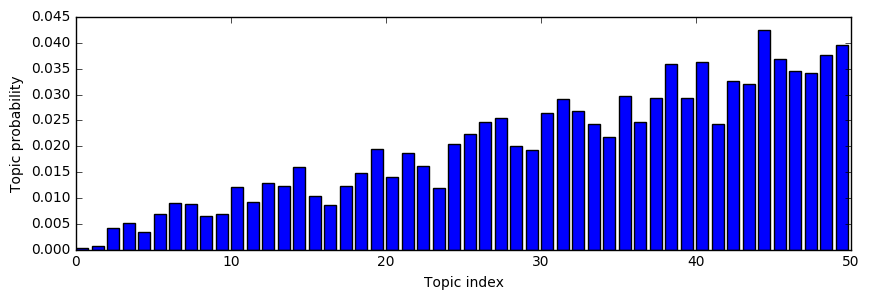
\includegraphics[scale=0.65]{3.png}
	\caption{Веса всех $50$ классов равномерно возрастают: $\alpha_i = i$}
	\label{fig:dir_inc_w}
	\end{figure}
		\item заметим, что если веса всех классов достаточно большие (и $>1$), то в силу наличия квадрата суммы весов в выражении дисперсии (\ref{dir_var}) для распределения Дирихле, эта дисперсия стремиться к нулю, а значит итоговые вероятности, сгенерированные $Dir(\alpha)$ будут близки к своим ожидаемым значениям! К примеру, на графике~\ref{fig:eq_w_dir} показан случай, когда веса всех классов одинаковы и большие. Получаем равномерное распределение.
	\begin{figure}[ht!]
	\centering
	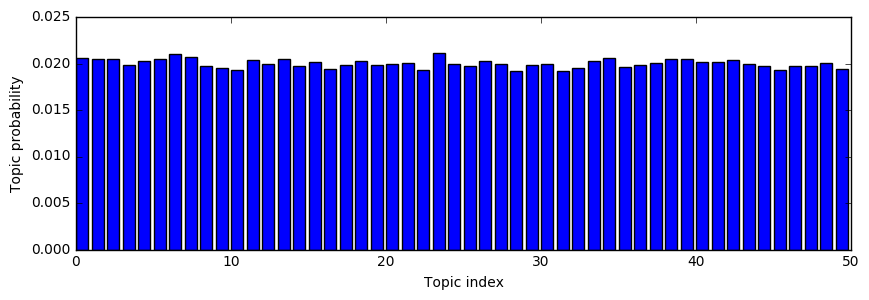
\includegraphics[scale=0.65]{1.png}
	\caption{Веса всех $50$ классов одинаковы и равны $1000$}
	\label{fig:eq_w_dir}
	\end{figure}
		\item Что будет, если веса наоборот малы (всяко $< 1$)? Посмотрим теперь на то, как будет распределена вероятность. Функция плотности Дирихле: 
		$Dir(\vec{p} | \vec{\alpha}) = \frac{1}{B(\vec{\alpha})}\prod_{i = 1}^{m}{p_i^{\alpha_i - 1}}$. При каких $\vec{p}$ в случае малых весов эта функция максимальна? Если $\alpha_i < 1$, то $\alpha_i - 1 < 0$. Тогда можно записать плотность так:
		\begin{equation*}
			Dir(\vec{p} | \vec{\alpha}) = \frac{1}{B(\vec{\alpha})}\prod_{i = 1}^{m}{\frac{1}{p_i^{\gamma_i}}}
		\end{equation*}
		Тут $\gamma_i$ > 0, $\frac{1}{B(\vec{\alpha})}$ --- константа. Видно, что плотность больше в тех $\vec{p}$, где больше близких к нулю компонент (т.к. если $p_i \rightarrow 0$, то $\frac{1}{p_i^{\gamma_i}} \rightarrow \infty$). Таким образом, при $\alpha \rightarrow 0$ мы будем получать, что вероятности очень разреженно распределяются, как показано на рисунке~\ref{fig:dir_small_w}. Чем ближе у нулю $\alpha_i$, тем меньше отличных от нуля (близких к нулю) $p_i$ на выходе.
	\begin{figure}[ht!]
	\centering
	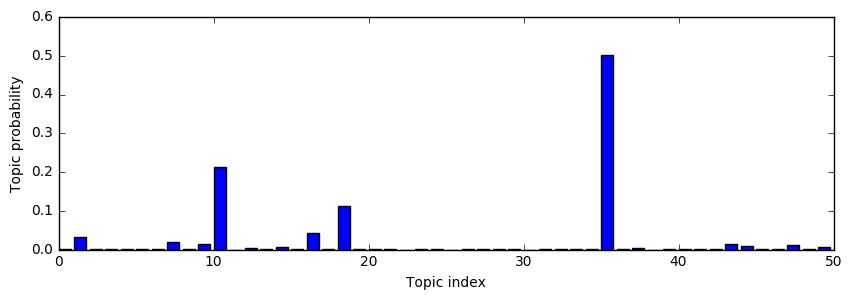
\includegraphics[scale=0.65]{2.png}
	\caption{Веса всех $50$ классов одинаковы и равны $0.07$}
	\label{fig:dir_small_w}
	\end{figure}
		\item Замечание: функция плотности распределения Дирихле, на самом деле, будет иметь один глобальный максимум, при $\alpha_i > 1$, который находится в точке $E[\vec{p}]$ (это к обоснованию первых двух пунктов объяснения).
	\end{itemize} 

	\item Какие значения этих параметром имеет смысл использовать и почему? Наверное, это зависит от конкретной коллекции документов. Но:
	\begin{itemize}
		\item Наверное мы предполагаем, что темы как-то более или мене равномерно распределены по документам, т.е. нет перекоса на какую-то тему. В тематической модели мы выбираем тему для каждого слова документа. При этом вряд ли бывают документы, которые содержат в себе больше какого-то разумного предела тем (например, пяти). По-этому стоит выбирать вектор параметров $\alpha$, исходя из предыдущего пункта задания, таким, что $\alpha_i$ малы (до нужной степени), дабы получать разреженные распределения тем в документе (как на рисунке~\ref{fig:dir_small_w}).
		\item При наличии какого-то априорного знания о том, что в коллекции превалирует определённое множество тем, можно соответствующим образом поднять веса $\alpha_i$ этих тем
		\item Как быть с параметрами $\vec{\beta}$, которые отвечают за распределение слов в теме. Тут ситуация похожая. Думаю, что для начала можно просто задать равномерное распределение, т.е. задать равные веса $\alpha_i$ и в зависимости от степени нашей уверенности делать их по модулю больше или меньше. Аналогично предыдущему пункту можно добавить перекос в сторону более частых слов при помощи увеличивания весов.
	\end{itemize}
\end{itemize}
\end{solution}

\begin{task}[3]
В дополнение к переходам по гиперссылкам пользователь может кликать <<назад>>. Можно ли и как смоделировать это марковской цепью? Как смоделировать повторяющиеся щелчки по кнопке <<назад>>?
\end{task}
\begin{solution}
Вообще марковские цепи представляются матрицей вероятностей переходов и в каждый момента времени решение о новом переходе производится исключительно исходя из текущего состояния, не используя информацию о том, каким путём мы добрались до этого состояния (это неформальное определение свойства Маркова для последовательности случайных величин), поэтому хочется ответить, что смоделировать, используя то же пространство состояний (состояние == документ), <<нельзя>>...
\begin{itemize}
	\item (1) Простая мысль: может быть, используя тот же web-граф, пускай от документа $B$ есть $m$ гиперссылок на $m$ других документов $A_i$. Давайте считать, что кнопка назад --- это ещё одна гиперссылка ($m+1$-ая), которая равновероятно может привести нас в любой из документов $D_i$, что в web-графе есть ребро $(D_i, B)$. В целом, это будет абсолютно допустимая модель, которую можно обосновать так: периодически пользователь может перескочить на какой-то случайных документ (как при телепортации, что обсуждалась на лекциях), только вероятность перескочить на странички, из которых достижима текущая, больше. Таким образом вероятности переходов из документа $B$ будут следующими (с учётом телепортаций):
	\begin{align*}
		p(B\rightarrow A_i) &= (1-\alpha)\xparen{\frac{1}{out(B) + 1}} + \alpha\frac{1}{N}\\
		p(B\rightarrow D_i) &= (1-\alpha)\frac{1}{(out(B)+1)\cdot in(B)} + \alpha\frac{1}{N}
	\end{align*}
	В некотором роде, это учитывает переходы назад, но совсем не точно, как бы хотелось.

	\item (1) Вариант два: будем менять граф состояний! У нас был граф из состояний-документов $\xbrace{D_1, D_2, \ldots, D_n}$ с какими-то гиперссылками $D_i \rightarrow D_j$. Давайте добавим фиктивную вершину $S$ (она обозначает начальную страницу браузера, с которой начинается поиск и с которой нельзя уйти назад) и добавим следующие вершины:
	\begin{align*}
		&[S,D_i] \text{ для всех вершин } D_i  \\
		&[D_i, D_j] \text{ для всех вершин } D_i,D_j; \text{ (вынуждены для всех из-за телепортаций =/)} 
	\end{align*}
	Новую матрицу смежности заполняем так:
	\begin{equation*}
		\text{Если } A(D_i, D_j) = 1, \text{ то } \forall X \in \xbrace{D_1, \ldots, D_n, S}\ A([X,D_i], [D_i, D_j]) = 1
	\end{equation*}
	А так же поддерживаем клики по кнопке назад:
	\begin{equation*}
		\text{Если } A([B,C], [С,E]) = 1, \text{ то } A([С,E], [S,C]) = 1
	\end{equation*}
	Замечу, что тут моделируется ровно один клик назад (т.к. переход по нему инвалидирует кнопку назад), иначе, если бы вместо вершины $[S,C]$ использовалась $[B,C]$, то получалось, что мы как бы неявно учитываем ещё какую-то историю предыдущих посещений (в данном случае элемент $B$).

	Вероятности переходов для марковской цепи считаются абсолютно аналогично случаю, рассмотренному на лекции. С одним но: телепортация из вершины $[D_i, D_j]$ может происходить только в вершину вида $[D_j, X]$.

	\item (2) Как поддержать последовательность кликов назад? Если нам интересно поддержать фиксированное число кликов, то можно использовать тот же подход, что и в пункте выше, но уже у нас будут и пары и тройки и т.д. пока нам интересно. Минус в том, что комбинаторный взрыв.
\end{itemize}
\end{solution}

\begin{task}[4]
Основная идея метода Ranking SVM. Что оптимизирует этот метод? Какие данные использует для обучения и как их получить?
\end{task}
\begin{solution}
\begin{itemize}
	\item Метод Ranking SVM для обучения использует пары $(q, r*)$, где $q$ --- это запрос, а $r*$ --- это ранжирование, представленное в следующем виде: $r*$ состоит из пар документов $(d_i, d_j)$, причём $(d_i, d_j)\in r*$, если документ $d_i$ имеет более высокий ранк (он <<лучше>>), чем документ $d_j$. При обучении пары запрос-документ переводятся в пространство признаков $(q, d) \rightarrow \Phi(q, d)$. А обучаемая функция ранжирования $f_{\omega}$ такова, что $(d_i, d_j)\in f_{\omega}(q)$ iff $\vec{\omega}\Phi(q, d_i) > \vec{\omega}\Phi(q, d_j)$.
	\item Как эти данные получить? Например, обратиться к LETOR (Microsoft Research Learning To Rank datasets), Yahoo! LETOR dataset, Интернет-математика — 2009 yandex dataset. В перечисленных датасетах есть оценки релевантности от асессоров, так что пары для обучения построить можно.
	\item Основная идея. Общая задача заключается в том, чтобы обучить такую функцию ранжирования $f(q)$ из семейства линейных функций с параметрами (вектор коэффициентов) $\omega$, что математическое ожидание метрики ранжирования $\tau(r*, r_{f(q)})$ максимально (математическое ожидание на распределении запросов и их идеальных ранжирований, т.е. на распределении входного датасета), где $r_{f(q)}$ --- ранжирование, полученное при помощи нашей обученной функции. Метрика $\tau$ такова:
	\begin{equation*}
		\tau(r_a, r_b) = \frac{P-Q}{P+Q} = 1 - \frac{2Q}{{m \choose 2}}
	\end{equation*}
	Тут $P$ --- это число пар $(d_i, d_j)$ которые принадлежат обоим ранжированиям, а $Q$ --- это число пар, в которых ранжирования расходятся, т.к. $(d_i, d_j) \in r_a$, но $(d_j, d_i) \in r_b$.
	Собственно далее решаются задачи оптимизации...
\end{itemize}
\end{solution}

\begin{task}[5]
Объясните ZScore и Sum нормировки с точки зрения предполагаемого статистического распределения нормируемых данных. Какие распределения предполагают эти методы и что они делают с предполагаемыми распределениями?
\end{task}
\begin{solution}
\begin{itemize}
	\item Z-Score. Это просто линейное преобразование распределения. Первым делом, вычитая математическое ожидания (среднее) мы получаем новую случайную величину, математическое ожидание которой $= 0$ и это будет работать в силу линейности матожидания для любого распределения. Далее мы делим на среднеквадратичное отклонения (корень дисперсии), что на нулевое матожидание никак не влияет, а вот по свойству дисперсии случайной величины (множитель вынесется с квадратом) получи, что новая случайная величина будет иметь дисперсию $=1$. С точки зрения статистического распределения мы в этих нормировках используем статистики, посчитанные по выборке, а не реальные значения моментов генеральной совокупности :) Итого, ZScore предполагает произвольное распределение и сохраняет его.
	\item Sum. $s' = s - min,\ s_n = \frac{s'}{\sum{s'_i}}$ Такое преобразование, кажется, уже не сохраняет вообще говоря исходное распределение. С точки зрения статистики мы получаем набор значений, которые суммируются в единицу и минимальным имеют 0, т.е. по сути являют собой вероятности. Про конкретные виды распределений сказать ничего не могу =( Но кажется разумным, что такой нормализатор нужно использовать с распределениями, с большей вероятностью сэмплирующими большие числа =)
\end{itemize}
\end{solution}

\begin{task}[6]
Про expert finding
\end{task}
\begin{solution}
\begin{itemize}
	\item Кажется, что для этой задачи хорошо подходят тематические модели (LDA и пр.). Для поддержки поиска экспертов нам понадобится связать каждый документ с его автором (экспертом). Далее, для каждого документа нужно построить тематическую модель этого документа. Так проанализировав все доступные документы для каждого эксперта мы можем построить тематическую модель эксперта просто с весами взвесив модели документов (mixture!) или как-то похожим образом. При получении запроса от пользователя мы используем подход, как я понимаю, из языковых моделей и в качестве результата и находим наиболее правдоподобные модели экспертов для запроса. Вуаля. Тут можно так же добавить ранжирование по числу документов (если это магическим образом не учтётся в смеси моделей) у эксперта, по его цитируемости и прочее.
	\item Почему бы не попробовать обычный полнотекстовый поиск с ранжированием (bm-25, например), но отобразить результирующий набор документов в набор экспертов, просто введя некую ранжирующую функция в духе: рейтинг эксперта --- это число документов за авторством конкретного эксперта в выдаче делить на сумму позиций в ранжировании, полученном на первом шаге.
	\item Опять же, идея похожая на тематические модели. Но теперь составим просто языковую модель каждого эксперта. Тут хорошо то, что мы можем просто взять и склеить все статьи и письма и прочее одного эксперта в один большой текст. Это позволит построить хорошую языковую модель, т.к. склейка получится достаточно большой (вероятно). Далии просто устраивать поиск и находить по запросу наиболее похожую к нему модель.
\end{itemize}
\end{solution}

\begin{task}[7]
Формулы полной вероятности и условной вероятности клика для PBM.
\end{task}
\begin{solution}
Насколько я понял, то полную вероятность клика мы получали на лекции:
\begin{equation*}
P(C_u = 1) = P(E_{r_u} = 1)P(A_u=1) = \gamma_{r_u} \alpha_{uq}
\end{equation*}
Тут $A_u$ --- привлекательность документа (привлекателен или нет), а $E_{r_u}$ --- сл. вел. обозначающая, наблюдал ли пользователь этот документ (examination).
Условные вероятности:
\begin{align*}
	P(C_u = 1 | E_{r_u} = 1) &= \frac{P(C_u = 1)-P(C_u = 1 | E_{r_u} = 0)P(E_{r_u} = 0)}{P(E_{r_u} = 1)} = \frac{P(C_u = 1)}{P(E_{r_u} = 1)} = P(A_u=1)\\
	P(C_u = 1| A_u = 1) &= \text{аналогично} = P(E_{r_u}=1)
\end{align*}
Я не очень понимаю, что тут можно объяснять, т.к. это всё следует из условия: 
\begin{equation*}
C_u = 1 \iff A_u = 1 \land E_{r_u} = 1
\end{equation*}
\end{solution}
\end{document}
